\documentclass{school}
\title{Entwurfsmuster}
\subject{Softwareentwicklung}
\author{Markus Reichl}

\begin{document}
\maketitle
\thispagestyle{fancy}
\tableofcontents

\section{Einführung}
Entwurfsmuster in der Softwareentwicklung bieten Lösungen zu wiederkehrenden Problemen im Software Design. Es handelt sich dabei nicht um fertige Implementierungen, sondern um Vorlagen, welche je nach Situation angepasst werden.

\subsection{Warum Entwurfsmuster?}
Entwurfsmuster beschleunigen den Entwicklungsprozess und verhindern Probleme, die sonst erst am Ende der Entwicklung zum Vorschein kommen und schwere Folgen nach sich ziehen.

Zusätzlich können Muster dazu verwendet werden um die Kommunikation zwischen Entwicklern zu verbessern, da diese allgemein bekannt, leicht verständlich und allgemein erweiterbar sind.

\section{Kategorien}
Es gibt unterschiedliche Typen von Entwurfsmustern, welche in 3 konkrete Typen unterschieden wurden. Hierzu ein paar Beispiele.

\begin{tabularx}{\textwidth}{X | X | X}
\textbf{Erzeugungsmuster} & \textbf{Strukturmuster} & \textbf{Verhaltensmuster}\\
\hline
Abstrakte Fabrik & Dekorierer & Beobachter\\
Einzelstück & Stellvertreter & Strategie\\
Fabrikmethode & & Besucher
\end{tabularx}
\vspace{0.5em}~\\
Mittlerweile reicht diese Einteilung nicht mehr aus um alle Entwurfsmuster zu kategorisieren. Weitere Muster sind zum Beispiel MCV, MVP, MVVM, DAO Muster.

\newpage
\section{Dekorierer}
\begin{figure}[h]
	\centering
	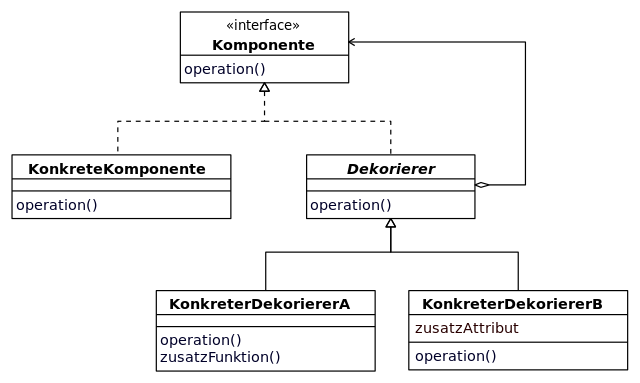
\includegraphics[height=4cm]{decorator.png}
	\caption{UML Dekorierer \cite{wiki-dekorierer-uml}}
\end{figure}

"Die Instanz eines Dekorierers wird vor die zu dekorierende Klasse geschaltet. Der Dekorierer hat die gleiche Schnittstelle wie die zu dekorierende Klasse. Aufrufe an den Dekorierer werden dann verändert oder unverändert weitergeleitet (Delegation), oder sie werden komplett in Eigenregie verarbeitet. Der Dekorierer ist dabei „unsichtbar“, da der Aufrufende gar nicht mitbekommt, dass ein Dekorierer vorgeschaltet ist."\\ $-$ Wikipedia \cite{wiki-dekorierer}

\subsection{Vor- und Nachteile}
\paragraph{Vorteile}

\begin{outline}
\1 Mehrere Dekorierer können hintereinandergeschaltet werden. 
\1 Dekorierer können zur Laufzeit und nach der Instanziierung ausgetauscht werden.
\1 Die zu dekorierende Klasse wird nur anhand ihrer Schnittstelle festgelegt.
\1 Lange und unübersichtliche Vererbungshierarchien werden vermieden.
\end{outline}

\paragraph{Nachteile}
\begin{outline}
\1 Dekorierte Komponenten müssen anhand ihrer Schnittstelle getestet werden.
\1 "Bei der Verwendung von dekorierten Komponenten müssen die Nachrichten vom Dekorierer an das dekorierte Objekt weitergeleitet werden."\\ $-$ Wikipedia \cite{wiki-dekorierer}
\end{outline}

\newpage
\section{Abstrakte Fabrik}
\begin{figure}[h]
	\centering
	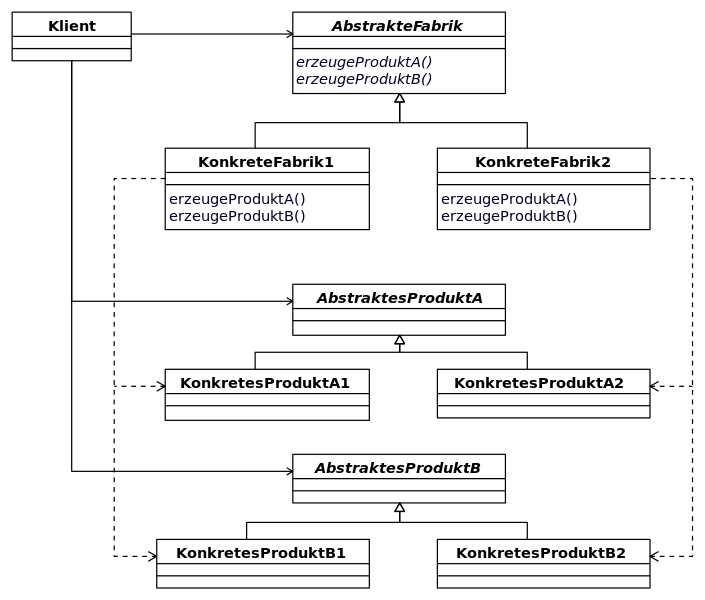
\includegraphics[height=6cm]{abstractfactory.png}
	\caption{UML Abstrakte Fabrik \cite{wiki-abstraktefabrik-uml}}
\end{figure}
~\\
"Die abstrakte Fabrik wird angewendet, wenn
\begin{outline}
\1 ein System unabhängig von der Art der Erzeugung seiner Produkte arbeiten soll,
\1 ein System mit einer oder mehreren Produktfamilien konfiguriert werden soll,
\1 eine Gruppe von Produkten erzeugt und gemeinsam genutzt werden soll oder
\1 wenn in einer Klassenbibliothek die Schnittstellen von Produkten ohne deren Implementierung bereitgestellt werden sollen.
\end{outline}
Eine typische Anwendung ist die Erstellung einer grafischen Benutzeroberfläche mit unterschiedlichen Oberflächenmotiven. Eine abstrakte Fabrik vereinigt die Verantwortlichkeiten „Zusammenfassung der Objektgenerierung an einer Stelle“ und „Möglichkeit zu abstrakten Konstruktoren“ (siehe auch unten unter „Verwandte Entwurfsmuster“)."\\
$-$ Wikipedia \cite{wiki-abstraktefabrik}

\subsection{Vor- und Nachteile}
\paragraph{Vorteile}
\begin{outline}
\1 Der Klient ist von konkreten Klassen isoliert.
\1 Der Austausch von Produktfamilien ist auf einfache Art und Weise möglich.
\end{outline}

\paragraph{Nachteile}~\\
"Neue Produktarten lassen sich schwer hinzufügen, da in allen konkreten Fabriken Änderungenvorzunehmen sind."
$-$ Wikipedia \cite{wiki-abstraktefabrik}

% Basic bibiography
\newpage
\begin{thebibliography}{9}
\bibitem{wiki-muster} Wikipedia, Entwurfsmuster \\ https://de.wikipedia.org/wiki/Entwurfsmuster
\bibitem{sourcemaking-designpatterns} Sourcemaking, Design Patterns \\ https://sourcemaking.com/design\_patterns
\bibitem{wiki-dekorierer-uml} Wikipedia Commons, Dekorierer \\ https://upload.wikimedia.org/wikipedia/commons/thumb/6/69/Dekorierer.svg/640px-Dekorierer.svg.png
\bibitem{wiki-dekorierer} Wikipedia, Dekorierer \\ https://de.wikipedia.org/wiki/Decorator
\bibitem{wiki-abstraktefabrik-uml} Wikipedia Commons, Abstrakte Fabrik \\ https://upload.wikimedia.org/wikipedia/commons/thumb/0/02/AbstkrakteFabrik.svg/705px-AbstkrakteFabrik.svg.png
\bibitem{wiki-abstraktefabrik} Wikipedia, Abstrakte Fabrik \\ https://de.wikipedia.org/wiki/Abstrakte\_Fabrik
\end{thebibliography}
\end{document}
